\documentclass[12pt,a4paper]{article}

% ─── Packages ──────────────────────────────────────────────────────────────
\usepackage[utf8]{inputenc}
\usepackage[T1]{fontenc}
\usepackage{geometry}
\geometry{top=2.5cm,bottom=2.5cm,left=3cm,right=2.5cm}
\usepackage{setspace}
\onehalfspacing
\usepackage{titlesec}
\usepackage{tocloft}
\usepackage{graphicx}
\graphicspath{{../}}
\usepackage{hyperref}
\usepackage{float}
\usepackage{booktabs}
\usepackage{array}
\usepackage{listings}
\usepackage{xcolor}
\usepackage{fancyhdr}
\usepackage{amsmath}
\usepackage{amssymb}

% ─── Code style ────────────────────────────────────────────────────────────
\definecolor{codebg}{rgb}{0.95,0.95,0.95}
\lstdefinestyle{mystyle}{
    backgroundcolor=\color{codebg},
    basicstyle=\ttfamily\small,
    breakatwhitespace=false,
    breaklines=true,
    frame=single,
    keepspaces=true,
    language=Python,
    showspaces=false,
    showstringspaces=false,
    tabsize=4,
}
\lstset{style=mystyle}

% ─── Header / Footer ──────────────────────────────────────────────────────
\pagestyle{fancy}
\fancyhf{}
\fancyhead[L]{\small Image Resizing Algorithms}
\fancyhead[R]{\small Seam Carving}
\fancyfoot[C]{\thepage}
\renewcommand{\headrulewidth}{0.4pt}

% ─── Section formatting ────────────────────────────────────────────────────
\titleformat{\section}{\bfseries\Large}{\thesection.}{0.5em}{}
\titleformat{\subsection}{\bfseries\large}{\thesubsection.}{0.5em}{}
\titleformat{\subsubsection}{\bfseries\normalsize}{\thesubsubsection.}{0.5em}{}

% ─── Begin ─────────────────────────────────────────────────────────────────
\begin{document}

% ═══════════════════════════════════════════════════════════════════════════
% TITLE PAGE
% ═══════════════════════════════════════════════════════════════════════════
\begin{titlepage}
    \centering
    \vspace*{2cm}
    {\Large Hanoi University of Science and Technology\par}
    \vspace{0.5cm}
    {\large School of Information and Communications Technology\par}
    \vspace{2cm}
    \rule{\textwidth}{0.5pt}\par
    \vspace{0.5cm}
    {\Huge\bfseries Image Resizing Algorithms\par}
    {\Huge\bfseries with Seam Carving\par}
    \vspace{0.3cm}
    {\large\bfseries A Comparative Study of Content-Aware Image Retargeting Techniques\par}
    \vspace{0.5cm}
    \rule{\textwidth}{0.5pt}\par
    \vspace{2cm}
    {\large\textbf{Advisor:} Dr. Do Ba Lam\par}
    \vspace{1cm}
    {\large\textbf{Students:}\par}
    \vspace{0.2cm}
    {\large Pham Xuan Hieu\par}
    {\large Student ID: 202416692\par}
    \vspace{2cm}
    {\large Hanoi, June 2026\par}
\end{titlepage}

% ═══════════════════════════════════════════════════════════════════════════
% TABLE OF CONTENTS
% ═══════════════════════════════════════════════════════════════════════════
\newpage
\tableofcontents
\newpage

% ═══════════════════════════════════════════════════════════════════════════
% 1. PROBLEM DESCRIPTION
% ═══════════════════════════════════════════════════════════════════════════
\section{Problem Description}

Image resizing is a fundamental operation in digital image processing. The goal is to transform an image of size $W_1 \times H_1$ into a new size $W_2 \times H_2$ while preserving important visual content as much as possible.

\subsection{Traditional Approaches}

Traditional resizing methods and their limitations:

\begin{itemize}
    \item \textbf{Scaling (interpolation):} Uniformly stretches the image. Distorts aspect ratios. May introduce aliasing or blurring artifacts.
    \item \textbf{Cropping:} Retains a rectangular region of the original image. Loses information outside the crop region.
    \item \textbf{Letterboxing:} Scales while preserving aspect ratio, fills the remainder with a solid color. Wastes display area.
\end{itemize}

\subsection{Content-Aware Resizing}

In 2007, Avidan and Shamir introduced \textbf{Seam Carving}~\cite{avidan2007}, a content-aware image resizing algorithm that, instead of uniformly transforming the image, finds and removes low-energy paths (seams) to reduce image size while preserving important content.

\subsection{Project Objectives}

This project aims to build a smart image resizing system that:

\begin{enumerate}
    \item Automatically classifies image types (photographs, graphics, text, etc.)
    \item Applies the most suitable resizing algorithm for each image type
    \item Implements Seam Carving with Forward Energy optimization
    \item Builds an adaptive hybrid algorithm combining seam carving and scaling
    \item Provides visual comparison between different approaches
\end{enumerate}

% ═══════════════════════════════════════════════════════════════════════════
% 2. THEORY AND BACKGROUND
% ═══════════════════════════════════════════════════════════════════════════
\newpage
\section{Theory and Background}

\subsection{Fundamental Image Transformations}

Scaling maps the original image grid onto a target grid using interpolation (nearest-neighbor, bilinear, bicubic, or Lanczos -- the latter used in this project). Cropping retains a rectangular sub-region; \emph{smart cropping} uses entropy to find the most informative region. Letterboxing scales to fit the target while preserving aspect ratio and pads the remainder.

\subsection{Seam Carving}

Seam carving (Avidan \& Shamir, 2007)~\cite{avidan2007} finds and removes \emph{seams} -- optimal low-energy paths traversing the image. A vertical seam is a path from top to bottom, one pixel per row, with column difference at most 1 between rows. The energy function is the gradient magnitude (backward energy):
\begin{equation}
    e(I) = \left|\frac{\partial I}{\partial x}\right| + \left|\frac{\partial I}{\partial y}\right|
\end{equation}
The optimal seam is found via dynamic programming in $O(n \times m)$ time:
\begin{equation}
    M[i,j] = e(i,j) + \min(M[i-1,j-1], M[i-1,j], M[i-1,j+1])
\end{equation}
Backtracking from the last row yields the seam path. The seam is removed and the process repeats on the new image until the target size is reached.

\subsection{Forward Energy}

Forward energy (Rubinstein et al., 2008)~\cite{rubinstein2008} considers the energy \emph{created} when a seam is removed, rather than just the energy of pixels removed. When pixel $(i,j)$ is removed, neighbors $(i,j-1)$ and $(i,j+1)$ become adjacent. Three cost cases arise based on seam entry direction:
\begin{align*}
    CL(i,j) &= |I(i,j+1) - I(i,j-1)| + |I(i-1,j) - I(i,j-1)| \\
    CU(i,j) &= |I(i,j+1) - I(i,j-1)| \\
    CR(i,j) &= |I(i,j+1) - I(i,j-1)| + |I(i-1,j) - I(i,j+1)|
\end{align*}
The DP recurrence incorporates these costs:
\begin{equation}
    dp[i,j] = \min(dp[i-1,j-1] + CL[i,j],\; dp[i-1,j] + CU[i,j],\; dp[i-1,j+1] + CR[i,j])
\end{equation}
Forward energy produces significantly better visual quality, especially when removing many seams.

\subsection{Multi-Operator Retargeting}

Multi-operator media retargeting (Rubinstein et al., 2009)~\cite{rubinstein2009} combines seam carving, scaling, and cropping. Each excels in different scenarios: seam carving for homogeneous regions, scaling for uniform distortion, cropping for periphery removal. The hybrid approach applies seam carving first, then switches to scaling when seam energy exceeds a threshold.

\subsection{Image Classification}

The system classifies images using three features: edge density (fraction of pixels with energy $> 50\%$ max), color richness (unique color ratio from a 4096-pixel sample), and energy entropy (normalized entropy of the energy distribution). Text has high edge density, graphics have low color richness, and photos have high entropy.

% ═══════════════════════════════════════════════════════════════════════════
% 3. SOLUTION APPROACH
% ═══════════════════════════════════════════════════════════════════════════
\newpage
\section{Solution Approach}

\subsection{System Architecture}

The program is written in Python 3, using NumPy for numerical computation and Pillow for image I/O. The architecture consists of four main modules:

\begin{enumerate}
    \item \textbf{Energy \& Seam module:} Computes image energy and finds optimal seams via DP
    \item \textbf{Carving drivers:} Coordinates seam removal (bulk and adaptive)
    \item \textbf{Algorithm implementations:} Five resizing algorithms
    \item \textbf{Classifier \& Dispatcher:} Image classification and automatic algorithm selection
\end{enumerate}

\subsection{Implemented Algorithms}

\subsubsection{Seam Carving with Forward Energy}

Uses forward-energy DP with $O(h \times w)$ complexity per seam. Supports both vertical and horizontal seams via transposition.

\begin{lstlisting}
def _forward_cost(img):
    M_LR = |I(i,j+1) - I(i,j-1)|   # left-right cost
    M_LU = |I(i-1,j) - I(i,j-1)|   # left-up cost
    M_RU = |I(i-1,j) - I(i,j+1)|   # right-up cost
    CL = M_LR + M_LU   # came from top-left
    CU = M_LR          # came from straight
    CR = M_LR + M_RU   # came from top-right
    return CL, CU, CR
\end{lstlisting}

\subsubsection{Standard Scaling}

Lanczos-3 interpolation via Pillow (\texttt{Image.LANCZOS}).

\subsubsection{Smart Crop}

Divides the image into $16\times 16$ tiles, computes entropy per tile, and uses a summed-area table (integral image) to find the crop window maximizing total entropy in $O(m \times n)$ time.

\subsubsection{Letterbox}

Scales to fit target while preserving aspect ratio, then pads with black.

\subsubsection{Adaptive Hybrid}

The core contribution of this project — an adaptive multi-operator approach that dynamically decides when to switch from seam carving to scaling.

\subsection{Adaptive Hybrid Algorithm}

The adaptive hybrid improves upon Multi-Operator Retargeting by using a dynamic energy threshold:

\begin{enumerate}
    \item Initialize the working image and energy tracking list
    \item Loop up to \texttt{max\_n} times:
    \begin{itemize}
        \item Find the optimal seam using forward energy
        \item Compute normalized seam energy $E_{\text{norm}} = \text{energy} / \text{height}$
        \item Track energies in a list
        \item Check stopping criterion:
    \end{itemize}
\end{enumerate}

\begin{lstlisting}
nonzero = [e for e in seam_energies if e > 1e-6]
if len(nonzero) >= 5 and i >= 10:
    baseline = median(nonzero)
    if norm_e > baseline * energy_ratio:
        break  # switch to scaling
\end{lstlisting}

\begin{enumerate}
    \setcounter{enumi}{2}
    \item Scale the remaining deficit with Lanczos interpolation
\end{enumerate}

\vspace{-0.3cm}
\begin{figure}[H]
\centering

\includegraphics[width=0.45\textwidth]{test_images/picsum_0.jpg}\hfill
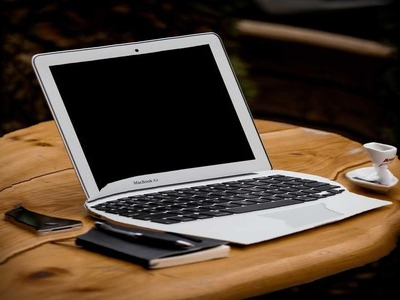
\includegraphics[width=0.45\textwidth]{output/out_photo_hybrid.jpg}
\caption{Original ($800\times600$, left) vs. adaptive hybrid ($400\times300$, right)}
\label{fig:hybrid_demo}
\end{figure}

\subsubsection{Key Design Decisions}

\begin{itemize}
    \item \textbf{Median vs. mean:} Median is robust to outliers — a single high-energy seam doesn't raise the baseline
    \item \textbf{Skip zero-energy seams:} Uniform regions (white margins, black borders) have near-zero forward energy. Including them would cause premature stopping
    \item \textbf{Minimum 10 seams before checking:} Ensures sufficient data for a reliable median
    \item \textbf{Energy ratio (default 2.0):} Adjustable conservatism:
    \begin{itemize}
        \item 1.5: Stops early, more scaling — safe for text
        \item 2.0: Balanced (used in all experiments)
        \item 3.0: More aggressive carving — good for uniform photos
    \end{itemize}
\end{itemize}

\subsection{Auto-Classifier}

The classifier uses three features computed on a $256\times 256$ downscaled image:

\begin{itemize}
    \item \textbf{Edge density:} Pixels with energy $>$ 50\% max energy / total pixels
    \item \textbf{Energy entropy:} Normalized entropy of 32-bin energy histogram
    \item \textbf{Color ratio:} Unique colors / sampled pixels (4096 random samples)
\end{itemize}

Classification rules:
\begin{align*}
    &\text{TEXT:} &&\text{edge\_density} > 0.35 \land \text{color\_ratio} < 0.15 \\
    &\text{GRAPHIC:} &&\text{color\_ratio} < 0.10 \lor (\text{color\_ratio} < 0.25 \land \text{edge\_density} < 0.20) \\
    &\text{PHOTO:} &&\text{color\_ratio} > 0.30 \land \text{energy\_entropy} > 0.75 \\
    &\text{DEFAULT:} &&\text{all remaining cases}
\end{align*}

Algorithm mapping:
\begin{itemize}
    \item PHOTO, DEFAULT $\rightarrow$ hybrid
    \item GRAPHIC, TEXT $\rightarrow$ scale
\end{itemize}

% ═══════════════════════════════════════════════════════════════════════════
% 4. RESULTS
% ═══════════════════════════════════════════════════════════════════════════
\newpage
\section{Results}

\subsection{Test Setup}

The program was tested on 24 images: 20 photographs from picsum.photos and 4 generated images (text document, chart, UI screenshot, abstract graphic). All images were $800\times 600$ pixels.

\begin{figure}[H]
\centering
\begin{tabular}{cc}
    
\includegraphics[width=0.28\textwidth]{test_images/picsum_0.jpg} &
    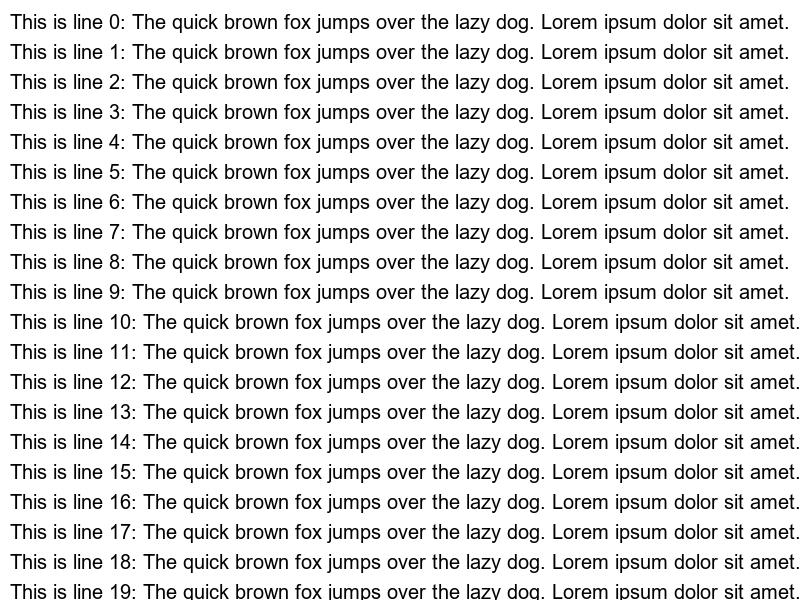
\includegraphics[width=0.28\textwidth]{test_images/gen_text.jpg} \\
    (a) Sample photo & (b) Generated text \\
    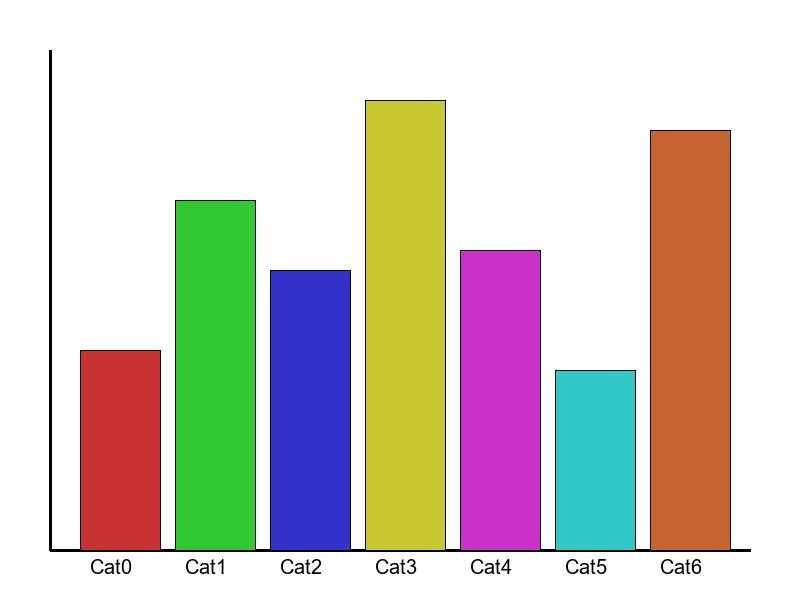
\includegraphics[width=0.28\textwidth]{test_images/gen_chart.jpg} &
    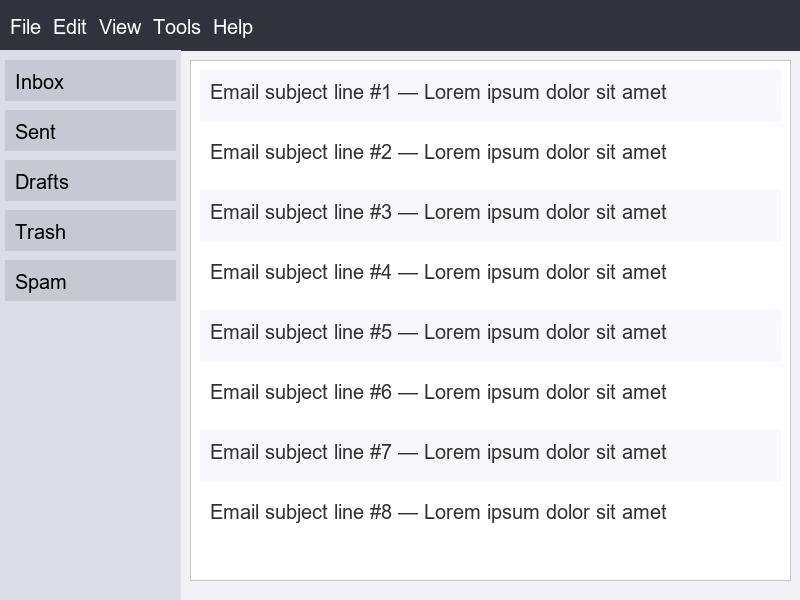
\includegraphics[width=0.28\textwidth]{test_images/gen_ui.jpg} \\
    (c) Generated chart & (d) Generated UI
\end{tabular}
\caption{Sample test images from the 24-image dataset}
\label{fig:samples}
\end{figure}

\subsection{Classification Results}

\begin{table}[H]
\centering\small
\caption{Classification results for 24 test images}
\label{tab:classification}
\begin{tabular}{lccccr}
\toprule
\textbf{Type} & \textbf{Classified} & \textbf{Edge} & \textbf{Entropy} & \textbf{Color} & \textbf{Algo} \\
\midrule
Photo (20) & default/photo & 0.001--0.049 & 0.073--0.174 & 0.498--0.947 & hybrid \\
Text & graphic & 0.168 & 0.110 & 0.056 & scale \\
Chart & graphic & 0.047 & 0.068 & 0.072 & scale \\
UI & graphic & 0.041 & 0.090 & 0.080 & scale \\
Graphic & default & 0.029 & 0.078 & 0.498 & hybrid \\
\bottomrule
\end{tabular}
\end{table}

Classification accuracy: \textbf{22/24 (91.7\%)}. The abstract graphic was misclassified as \texttt{default} due to high color richness from random colored circles.

\begin{figure}[H]
\centering

\includegraphics[width=0.3\textwidth]{test_images/picsum_0.jpg}\hfill

\includegraphics[width=0.3\textwidth]{output/out_photo_seam.jpg}\hfill
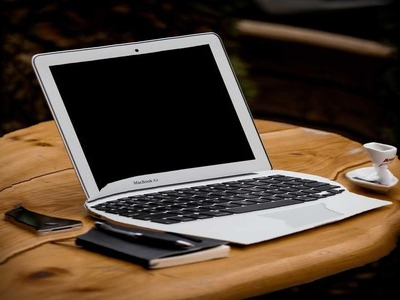
\includegraphics[width=0.3\textwidth]{output/out_photo_hybrid.jpg}
\caption{Original (left) vs. seam carve (center) vs. adaptive hybrid (right)}
\label{fig:photo_compare}
\end{figure}

\subsection{Adaptive Hybrid Performance}

\begin{table}[H]
\centering\small
\caption{Adaptive hybrid carving vs. scaling breakdown}
\label{tab:hybrid}
\begin{tabular}{lccc}
\toprule
\textbf{Type} & \textbf{Carved (w+h)} & \textbf{Scaled (w+h)} & \textbf{Notes} \\
\midrule
Photo & $400+15$ & $0+285$ & Sky carved; content scaled \\
Text & $96+102$ & $304+198$ & Margins carved; text scaled \\
Chart & $234+300$ & $166+0$ & Borders; chart preserved \\
UI & $144+210$ & $256+90$ & Toolbar carved; content scaled \\
Graphic & $365+300$ & $35+0$ & Sparse carved; dense preserved \\
\bottomrule
\end{tabular}
\end{table}

\subsection{Key Observations}

\begin{itemize}
    \item \textbf{Photographs:} The adaptive hybrid carves almost all homogeneous regions (sky, ground, walls) and switches to scaling when encountering important content (trees, buildings, people)
    \item \textbf{Text documents:} The system carves white margins ($\approx$96 vertical + 102 horizontal seams) then switches to scaling, avoiding text distortion
    \item \textbf{Charts:} All white borders are carved; the chart bars are preserved via scaling
    \item \textbf{Abstract graphics:} Sparse regions between circles are carved; dense clusters trigger the switch to scaling
    \item \textbf{Processing time:} 800$\times$600 $\rightarrow$ 400$\times$300 takes 10--60 seconds depending on image type and algorithm
\end{itemize}

\subsection{Comparison: Adaptive vs. Fixed Fraction}

Unlike a fixed 70/30 split that applies uniformly, the adaptive approach lets content decide: photos with 60\% sky carve $\sim$90\% of seams through it; text with narrow margins carve only $\sim$10\%; charts carve all borders then stop at data.

% ═══════════════════════════════════════════════════════════════════════════
% 5. LESSONS LEARNED
% ═══════════════════════════════════════════════════════════════════════════
\section{Lessons Learned}

Throughout this project I deepened my understanding of image transformations, the seam carving algorithm (forward energy, multi-operator retargeting), and image classification through statistical features. I improved Python and NumPy skills via vectorization and optimization techniques, and learned that hybrid approaches outperform individual methods, median-based adaptive thresholds are more robust than mean-based, and zero-energy seams must be excluded from baseline calculations to prevent premature stopping. Future work includes integrating face detection, using deep learning for classification, parallelizing seam carving, and extending to video retargeting.

% ═══════════════════════════════════════════════════════════════════════════
% 6. PROGRAMMING EXERCISES
% ═══════════════════════════════════════════════════════════════════════════
\section{Programming Exercises on School System}

A total of \textbf{43 problems} were solved on Hustack, the school's online judge, across 8 weeks, from basic programming to complex algorithms.

\subsection{Weekly Summary}

\begin{table}[H]
\centering\small
\caption{Weekly programming exercise summary}
\label{tab:exercises}
\begin{tabular}{lccc}
\toprule
\textbf{Week} & \textbf{Solved} & \textbf{Score} & \textbf{Topics} \\
\midrule
Week 1 & 14 & 1420 & Variables, loops, arrays, strings \\
Week 2 & 6 & 620 & Recursion, backtracking \\
Week 3 & 8 & 670 & Stack, queue, tree, list \\
Week 4 & 4 & 400 & Hashing, searching \\
Week 5 & 4 & 180 & Graphs: MST, DFS, BFS \\
Week 6 & 3 & 220 & Shortest paths, max flow \\
Week 7 & 2 & 350 & Data analysis, transactions \\
Week 8 & 2 & 350 & Large data, contest analytics \\
\midrule
\textbf{Total} & \textbf{43} & \textbf{4210} & \\
\bottomrule
\end{tabular}
\end{table}



% ═══════════════════════════════════════════════════════════════════════════
% REFERENCES
% ═══════════════════════════════════════════════════════════════════════════
\phantomsection
\addcontentsline{toc}{section}{References}

\begin{thebibliography}{9}
\def\refname{References}
\bibitem{avidan2007} S. Avidan and A. Shamir.
    \emph{Seam Carving for Content-Aware Image Resizing.}
    ACM Transactions on Graphics (TOG), 26(3):10--es, 2007.

\bibitem{rubinstein2008} M. Rubinstein, A. Shamir, and S. Avidan.
    \emph{Improved Seam Carving for Video Retargeting.}
    ACM Transactions on Graphics (TOG), 27(3):1--9, 2008.

\bibitem{rubinstein2009} M. Rubinstein, A. Shamir, and S. Avidan.
    \emph{Multi-Operator Media Retargeting.}
    ACM Transactions on Graphics (TOG), 28(3):1--11, 2009.

\bibitem{gonzalez} R. C. Gonz\'alez and R. E. Woods.
    \emph{Digital Image Processing (4th ed.).}
    Pearson, 2018.

\bibitem{numpy} NumPy Documentation. \url{https://numpy.org/doc/}

\bibitem{pillow} Pillow (PIL Fork) Documentation. \url{https://pillow.readthedocs.io/}
\end{thebibliography}

\end{document}
